% cd ..\..\Users\NikitaSkybytskyi\Desktop\c3s2\numerical-analysis\lab\lab-5\tex
% cls && pdflatex report.tex && cls && pdflatex report.tex && start report.pdf
\documentclass[12pt, a4paper]{article}
\usepackage[T2A]{fontenc}
\usepackage[utf8]{inputenc}
\usepackage[english,ukrainian]{babel}
\usepackage{amsmath, amssymb}
\usepackage{verbatim}

\usepackage[top = 2 cm, left = 1 cm, right = 1 cm, bottom = 2 cm]{geometry}

\usepackage{float, graphicx}
\usepackage{amsthm}
\newtheorem{lemma}{Лема}
\newtheorem*{lemma*}{Лема}
\newtheorem{theorem}{Теорема}
\newtheorem*{theorem*}{Теорема}
\newtheorem{definition}{Визначення}
\newtheorem*{definition*}{Визначення}
\theoremstyle{definition}
\newtheorem{remark}{Зауваження}
\newtheorem*{remark*}{Зауваження}
\newtheorem{example}{Приклад}
\newtheorem*{example*}{Приклад}
\newtheorem{problem}{Задача}
\newtheorem*{problem*}{Задача}
\newtheorem{solution}{Розв'язок}
\newtheorem*{solution*}{Розв'язок}
\newtheorem{corollary}{Наслідок}
\newtheorem*{corollary*}{Наслідок}

\newcommand{\NN}{\mathbb{N}}
\newcommand{\RR}{\mathbb{R}}
\newcommand{\CC}{\mathbb{C}}
\newcommand{\HH}{\mathcal{H}}
\newcommand{\Min}{\displaystyle\min\limits}
\newcommand{\Max}{\displaystyle\max\limits}
\newcommand{\Sup}{\displaystyle\sup\limits}
\newcommand{\Sum}{\displaystyle\sum\limits}
\newcommand{\Prod}{\displaystyle\prod\limits}
\newcommand{\Int}{\displaystyle\int\limits}
\newcommand{\Iint}{\displaystyle\iint\limits}
\newcommand{\Lim}{\displaystyle\lim\limits}

\newcommand*\diff{\mathop{}\!\mathrm{d}}

\renewcommand{\bf}[1]{\textbf{#1}}
\renewcommand{\epsilon}{\varepsilon}
\renewcommand{\phi}{\varphi}

\DeclareMathOperator{\signum}{sign}
\DeclareMathOperator{\diam}{diam}
\DeclareMathOperator{\rang}{rang}
\DeclareMathOperator{\const}{const}
\DeclareMathOperator{\cond}{cond}
\DeclareMathOperator{\diagonal}{diag}

\numberwithin{equation}{section}

\setlength\parindent{0pt}
\allowdisplaybreaks

\newcommand{\cover}[2]{
\begin{center}
\hfill \break
	Міністерство освіти та науки України \\
	Київський національний університет імені Тараса Шевченка \\ 
	Факультет комп'ютерних наук та кібернетики \\
	Кафедра обчислювальної математики
\end{center}

\vfill 

\begin{center}
	\large{
		Звіт до лабораторної роботи №{#1} на тему: \\ 
		``{#2}''
	}
\end{center}

\vfill 

\begin{flushright}
	Виконав студент групи ОМ-3 \\
	Скибицький Нікіта
\end{flushright}

\vfill 

\begin{center}
    Київ, 2018 
\end{center}

\thispagestyle{empty} 
\newpage
}

\begin{document}

\cover{5}{Найкраще середньоквадратичне наближення}

\tableofcontents

\section{Постановка задачі}

Усі завдання будуть виконані для функції $f$ вигляду: \[ f(x) = \frac{|x - 4| + |x + 4|}{2}, \quad a = -10 \le x \le 10 = b. \] Також задамо $n = 4$, $m = 20$. У всіх підзадачах необхідно побудувати графіки функцій $f(x)$ та отриманого наближення, обчислити відхилення.

\subsection{Найкраще середньоквадратичне наближення}

Побудувати поліном найкращого середньоквадратичного наближення $Q_n(x)$ для функції $f(x)$ на проміжку $[a, b]$, вибравши в якості лінійно незалежних функцій систему функцій $\phi_i(x)$, для $i=\overline{0,n}$. Системи функцій які будуть розглянуті:
\begin{enumerate}
    % \item $\phi_i(x) = x^i$;
    \item $\phi_i(x) = T_i(x)$ --- поліноми Чебишова;
    % \item експоненційна;
    \item тригонометрична.
\end{enumerate}

\subsection{Метод найменших квадратів}

Функція $y = f(x)$ задана таблицею значень $y_0, y_1, \ldots, y_m$ у точках $x_0, x_1, \ldots, x_m$. Використовуючи метод найменших квадратів (МНК), знайти поліном $Q_n(x) = a_0 + a_1 \cdot x + \ldots + a_n \cdot x^n$ найкращого середньоквадратичного наближення оптимального степеня $n = n^\star$. За оптимальне значення $n^\star$ будемо вважати той степінь поліному, починаючи з якого величина \[ \sigma_n = \sqrt{\frac{1}{m - n} \cdot \sum_{k = 0}^m (Q_n(x_k) - y_k)^2} \] стабілізується або починає зростати.

\subsection{Кубічні згладжувальні сплайни}

Побудувати кубічний згладжувальний  сплайн для функції $f(x)$ на проміжку $[a, b]$ за її значеннями у вузлах $x_i = a + i \cdot h$, для $i = \overline{0, m}$, де $h = (b - a) / m$, а $m \gg n$.

\section{Теоретична частина}

\subsection{Найкраще середньоквадратичне наближення}

Наблизимо функцію $f: \HH \to \RR$ з гільбертового простору $\HH$ функціями зі скінченновимірного підпростору $M_n$ простору $\HH$. Скалярний добуток у просторі $\HH$ ми будемо позначати як $(u, v)$, відповідну норму -- як $\|u\| = \sqrt{(u, u)}$. \medskip

Нехай $\{\phi_i\}_{i=0}^\infty$ --- лінійно-незалежна система функцій $\HH \to \RR$. Розглянемо її скінченну підсистему $\{\phi_i\}_{i=0}^n$. Позначимо лінійну оболонку цієї підсистеми за $M_n \subset \HH$. \medskip

Нагадаємо визначення ЕНН $\Phi$: \[ \|f - \Phi\| = \sqrt{(f - \Phi, f - \Phi)} = \inf_{\phi \in M_n} \|f - \phi\|. \] Якщо $\Phi$ --- ЕНН, то $(f - \Phi, \phi) = 0$ для довільного $\phi \in M_n$, тому можна записати $f = \Phi + \psi$, де $\Phi \in M_n$, $\psi \in M_n^\perp$, тому будемо шукати наближення у вигляді \[ \Phi = \sum_{i = 0}^n c_i \cdot \phi_i. \]

Для виконання $(f - \Phi, \phi) = 0$ достатньо, щоб \[ (f - \Phi, \phi_j) = 0, \quad j = \overline{0, n}, \] що у свою чергу дає \[ \left(f - \sum_{i = 0}^n c_i \cdot \phi_i, \phi_j \right) = 0, \quad j = \overline{0, n}. \] Звідси маємо СЛАР на $c_i$: \[ \sum_{i=0}^n c_i \cdot (\phi_i, \phi_j)_\rho = (f, \phi_j)_\rho, \quad j = \overline{0, n}. \]

Матриця цієї СЛАР --- $G = \|g_{ij}\|_{i,j=1}^{n}$, де $g_{ij} = (\phi_i, \phi_j)_\rho$ --- матриця Грамма лінійно-незалежної системи функцій $\{\phi_i\}_{i=0}^n$, що доводить існування та єдиність ЕНН. Оскільки $G^T = G$, то для роз\-в'яз\-у\-ва\-ння цієї СЛАР використовують метод квадратних коренів. У багатьох випадках матриця $G$ погано обумовлена, у цих випадках систему функцій вибирають ортогональною з ваговим коефіцієнтом $\rho$, де для поліномів Чебишова \[ \rho(x) = \frac{1}{\sqrt{1 - x^2}}. \]

Тоді СЛАР на $c_i$ набуває наступний вигляд:
\[ \begin{pmatrix} c_1 \\ c_2 \\ c_3 \\ \vdots \\ c_{n - 1} \\ c_n \end{pmatrix} \cdot \begin{pmatrix} (\phi_1, \phi_1)_\rho & 0 & 0 & \cdots & 0 & 0 \\ 0 & (\phi_2, \phi_2)_\rho & 0 & \cdots & 0 & 0 \\ 0 & 0 & (\phi_3, \phi_3)_\rho & \cdots & 0 & 0 \\ \vdots & \vdots & \vdots & \ddots & \vdots & \vdots \\ 0 & 0 & 0 & \cdots & (\phi_{n - 1}, \phi_{n - 1})_\rho & 0 \\ 0 & 0 & 0 & \cdots & 0 & (\phi_n, \phi_n)_\rho \end{pmatrix} = \begin{pmatrix} (f, \phi_1)_\rho \\ (f, \phi_2)_\rho \\ (f, \phi_3)_\rho \\ \vdots \\ (f, \phi_{n - 1})_\rho \\ (f, \phi_n)_\rho \end{pmatrix} \]

Явно запишемо розв'язок цієї СЛАР: \[ c_i = \frac{(f, \phi_i)_\rho}{(\phi_i, \phi_i)_\rho}, \] тоді \[ \Phi = \sum_{i = 0}^n \frac{(f, \phi_i)_\rho}{(\phi_i, \phi_i)_\rho} \cdot \phi_i, \] звідки у випадку ортонормованої системи функцій маємо наступний вираз відхилення: \[ \Delta^2(f) = \|f - \Phi\|^2 = \|f\| - \|\Phi\|^2 = \|f\| - \sum_{i=0}^n c_i^2.\] У випадку ортогональної але не нормалізованої системи відхилення шукається наступним чином: \begin{equation} \label{delta} \Delta^2(f) = \|f - \Phi\|^2 = \|f\| - \|\Phi\|^2 = \|f\| - \sum_{i=0}^n c_i^2 \cdot \|\phi_i\|^2. \end{equation}

\subsection{Метод найменших квадратів}

Нехай в результаті вимірювань функції $f(x)$ маємо таблицю значень: \[ y_i \approx f(x_i), \quad x_i \in [a, b], \quad i = \overline{0, m}.\] За даними цієї таблиці треба побудувати аналітичну формулу $\Phi(x; a_1, a_2, \ldots, a_n)$ таку, що \[ \phi(x_i; a_1, a_2, \ldots, a_n) \approx y_i, \quad i = \overline{0, m}.\] 

Розв'язувати цю задачу інтерполюванням (тобто задавати ``$=$'' замість ``$\approx$'') не раціонально, адже $m \gg n$ і отримана система буде перевизначена, її розв'язки як правило не існують. \medskip

Параметри $a_1, a_2, \ldots, a_n$ визначають з міркувань \[I(a_1, a_2, \ldots, a_n) = \sum_{i = 0}^m (y_i - \phi(x_i; a_1, a_2, \ldots, a_n)^2 \to \min,\] тому метод і називається методом найменших (суми) квадратів (відхилень). \medskip

Для досягнення мінімуму достатньо $\partial I / \partial a_i = 0$, для $i = \overline{0, n}$. Зокрема, якщо $\phi$ лінійно залежить від параметрів $a_1, a_2, \ldots, a_n$, то отримаємо СЛАР \[ \sum_{j = 0}^n a_j \cdot \phi_j(x_i) = y_i, \quad i = \overline{0, m},\] яку називають системою умовних рівнянь. \medskip

МНК рівносильний знаходженню ЕНН у гільбертовому просторі функцій $f: X \to \RR$ над дискретною множиною $X = \{x_0, x_1, \ldots, x_m\}$, у якому скалярний добуток визначається наступним чином: \[ (u, v) = \sum_{i = 0}^m u(x_i) \cdot v(x_i). \] Якщо відомі оцінки похибок $\epsilon_i$ для значень $y_i$ то скалярний добуток задають у вигляді \[ (u, v) = \sum_{i = 0}^m \frac{u(x_i) \cdot v(x_i)}{\epsilon_i^2}. \]

\subsection{Кубічні згладжувальні сплайни}

Розглянемо функціонал: \[ \Phi_1(u) = \Phi(u) + \sum_{i = 0}^n \rho \left( \tilde{f_i} - u(x_i) \right)^2,\] де $\rho_i > 0$ --- деякі числа, та \[\Phi(u) = \int_a^b (u''(x))^2 \diff x.\]

Згладжуючим сплайном назвемо функцію $g$, яка є розв'язком задачі: \[ \Phi_1(g) = \inf_{u \in W_2^2(a, b)} \Phi_1(u).\]

Позначимо \[ \mu_i = g(x_i), \quad i = \overline{0, n}, \quad m_i = g''(x_i), \quad i = \overline{1, n - 1}.\]

Позначимо: \[ A = \begin{pmatrix}
    1 & 0 & 0 & 0 & \cdots & 0 & 0 \\
    0 & \frac{h_1 + h_2}{3} & \frac{h_2}{6} & 0 & \cdots & 0 & 0 \\
    0 & \frac{h_2}{6} & \frac{h_2 + h_3}{3} & \frac{h_3}{6} & \cdots & 0 & 0 \\
    \vdots & \ddots & \ddots & \ddots & \ddots & \vdots & \vdots \\
    \vdots & \vdots & \ddots & \ddots & \ddots & \ddots & \vdots \\
    0 & 0 & \cdots & 0 & \frac{h_{n - 2}}{6} & \frac{h_{n - 2} + h_{n - 1}}{3} & \frac{h_{n - 1}}{6} \\
    0 & 0 & 0 & \cdots & 0 & \frac{h_{n - 1}}{6} & \frac{h_{n - 1} + h_n}{3} \\
    0 & 0 & 0 & 0 & \cdots & 0 & 1
\end{pmatrix} \]
а також
\[ H = \begin{pmatrix}
    0 & 0 & 0 & 0 & \cdots & 0 & 0 \\
    \frac{1}{h_1} & - \left( \frac{1}{h_1} + \frac{1}{h_2} \right) & \frac{1}{h_2} & 0 & \cdots & 0 & 0 \\
    0 & \frac{1}{h_2} & - \left( \frac{1}{h_2} + \frac{1}{h_3} \right) & \frac{1}{h_3} & \cdots & 0 & 0 \\
    \vdots & \vdots & \ddots & \ddots & \ddots & \vdots & \vdots \\
    \vdots & \vdots & \vdots & \ddots & \ddots & \ddots & \vdots \\
    0 & 0 & \cdots & 0 & \frac{1}{h_{n - 1}} & - \left( \frac{1}{h_{n - 1}} + \frac{1}{h_n} \right) & \frac{1}{h_n} \\
    0 & 0 & 0 & 0 & \cdots & 0 & 0
\end{pmatrix} \]

Якби значення $\mu_i$ були б відомі, то для побудови $g$ достатньо було б розв'язати систему \begin{equation} \label{amhmu} A \vec m = H \vec \mu \end{equation} та записати $g(x)$ за формулою:
\begin{multline} 
    \label{eq}
    g(x) = m_i \cdot \frac{(x_{i + 1} - x)^3}{6 h_i} + m_{i + 1} \cdot \frac{(x - x_i)^3}{6 h_i} + \\
    + \left( \mu_i - \frac{m_i \cdot h_i^2}{6} \right) \cdot \frac{x_{i + 1} - x}{h_i} + \left( \mu_{i + 1} - \frac{m_{i + 1} \cdot h_i^2}{6}\right) \cdot \frac{x - x_i}{h_i}, 
\end{multline}
де $x \in [x_i, x_{i + 1}]$, $h_i = x_{i + 1} - x_i$, $i = \overline{0, n - 1}$. \medskip

З умови мінімізації функціоналу $\Phi_1$ отримуємо систему рівнянь \[ 2 (H^T m)_i + 2 \rho_i (\mu_i - \tilde f_i) = 0. \] Позначимо $R = \diagonal \rho_i$ (діагональна матриця), тоді попередню формулу можна записати у матричному вигляді як \[ H^T \cdot \vec m + R \cdot \vec \mu = R \cdot \vec f.\] Помноживши зліва на $H \cdot R^{-1}$, отримаємо \[ H \cdot R^{-1} \cdot H^T \cdot \vec m + H \cdot \vec \mu = H \cdot \vec f. \] Враховуючи співвідношення \eqref{amhmu} маємо СЛАР на $m$: \[ (A + H \cdot R^{-1} \cdot H^T) \cdot \vec m = H \cdot \vec f.\] Після цього можемо знайти $\vec \mu$ за формулою: \[\vec \mu = \vec f - R^{-1} \cdot H^{T} \cdot \vec m.\] В результаті отримуємо сплайн що згладжує за формулою \eqref{eq}: \[ g(x) = m_i \cdot \frac{(x_{i + 1} - x)^3}{6 h_i} + m_{i + 1} \cdot \frac{(x - x_i)^3}{6 h_i} + \left( \mu_i - \frac{m_i \cdot h_i^2}{6} \right) \cdot \frac{x_{i + 1} - x}{h_i} + \left( \mu_{i + 1} - \frac{m_{i + 1} \cdot h_i^2}{6}\right) \cdot \frac{x - x_i}{h_i}, \] де $x \in [x_i, x_{i + 1}]$, $h_i = x_{i + 1} - x_i$, $i = \overline{0, n - 1}$.

\section{Практична частина}

\subsection{Найкраще середньоквадратичне наближення}

% \subsubsection{Степенева система функцій}
% \begin{figure}[H]
%     \centering
%     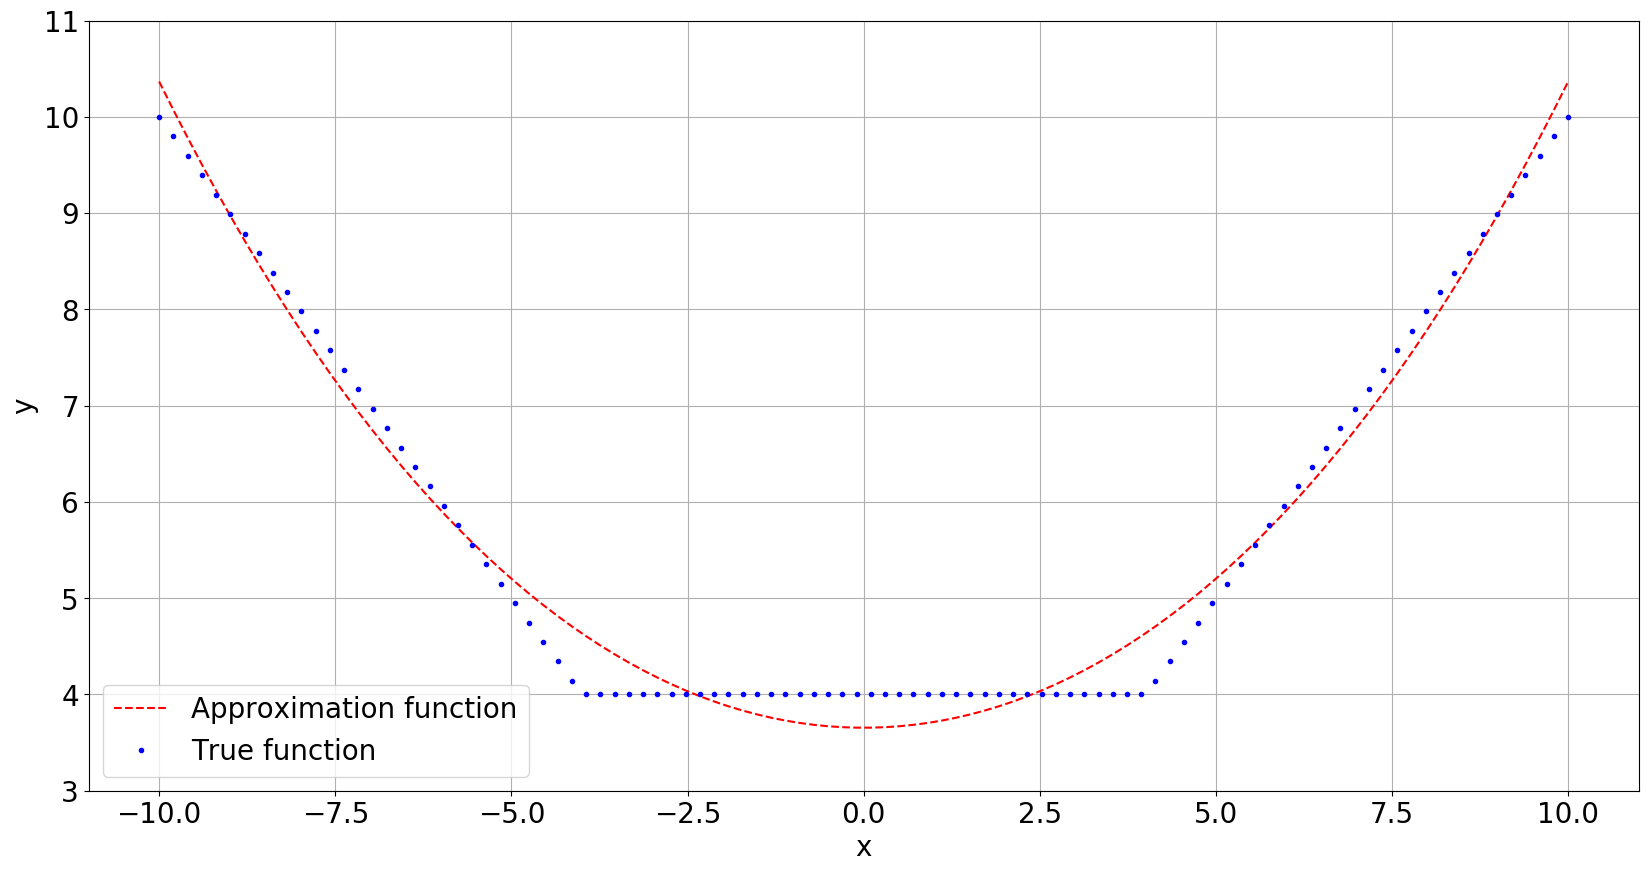
\includegraphics[width=\textwidth]{polynomial.png}
% \end{figure}
% \[ \Delta^2(f) = \texttt{1.3515894719986394}. \]

% \subsubsection{Експоненційна система функцій}
% \begin{figure}[H]
%     \centering
%     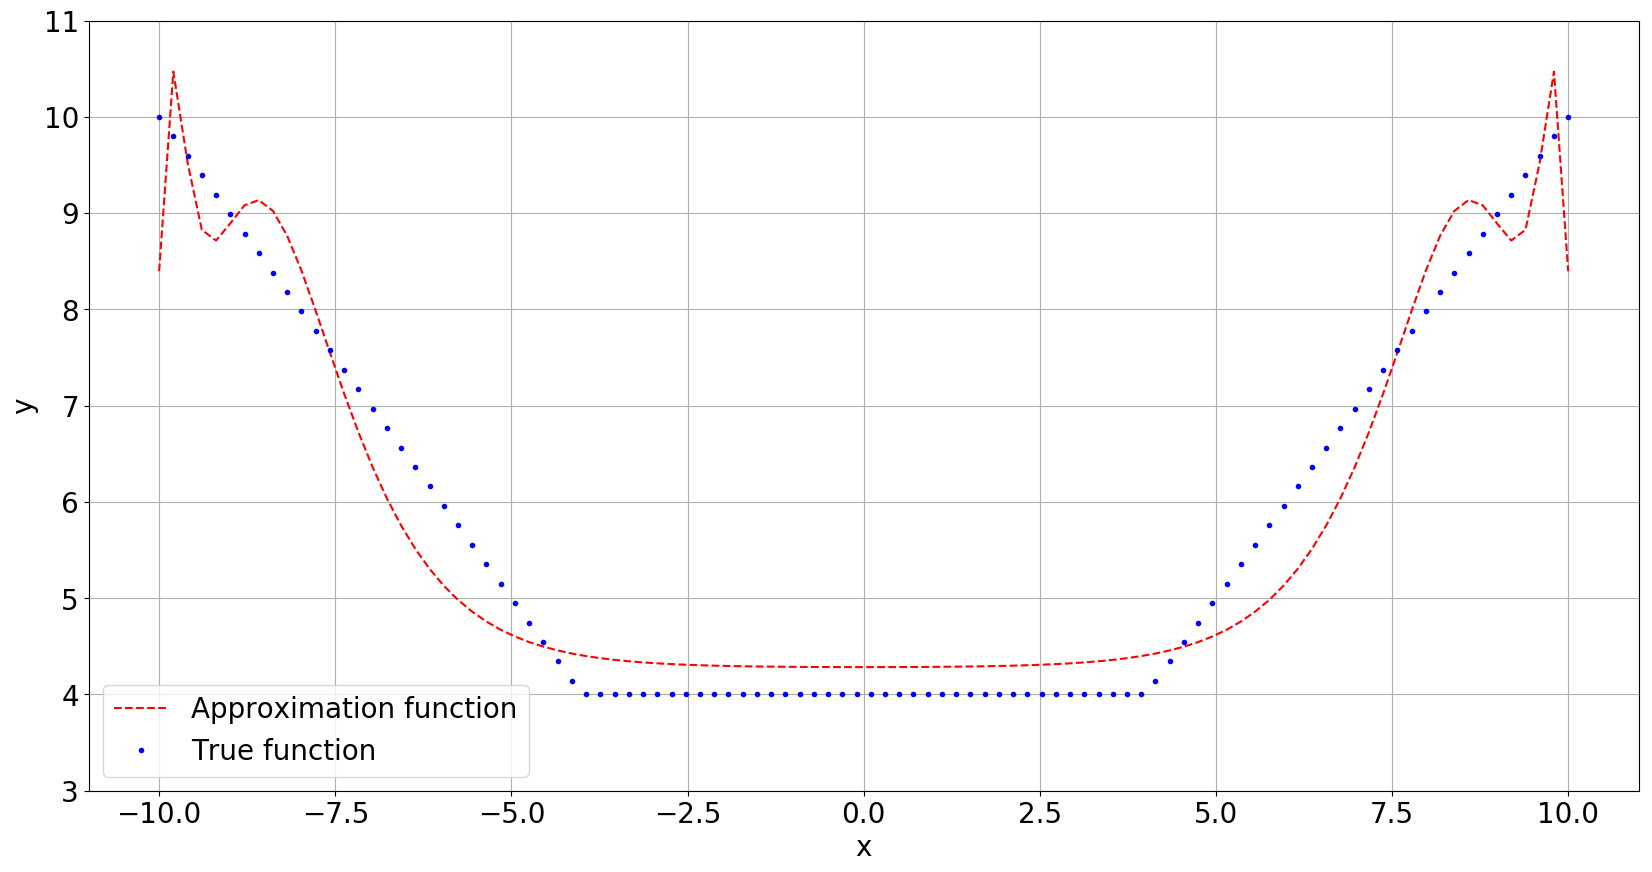
\includegraphics[width=\textwidth]{exponent.png}
% \end{figure}
% \[ \Delta^2(f) = \texttt{4.20306095641598}. \]

\subsubsection{Тригонометрична система функцій}

Система функцій $\{1, \sin x, \cos x, \sin 2x, \cos 2x, \ldots\}$, ортогональні без вагового множника на $[-\pi,\pi]$.

\begin{figure}[H]
    \centering
    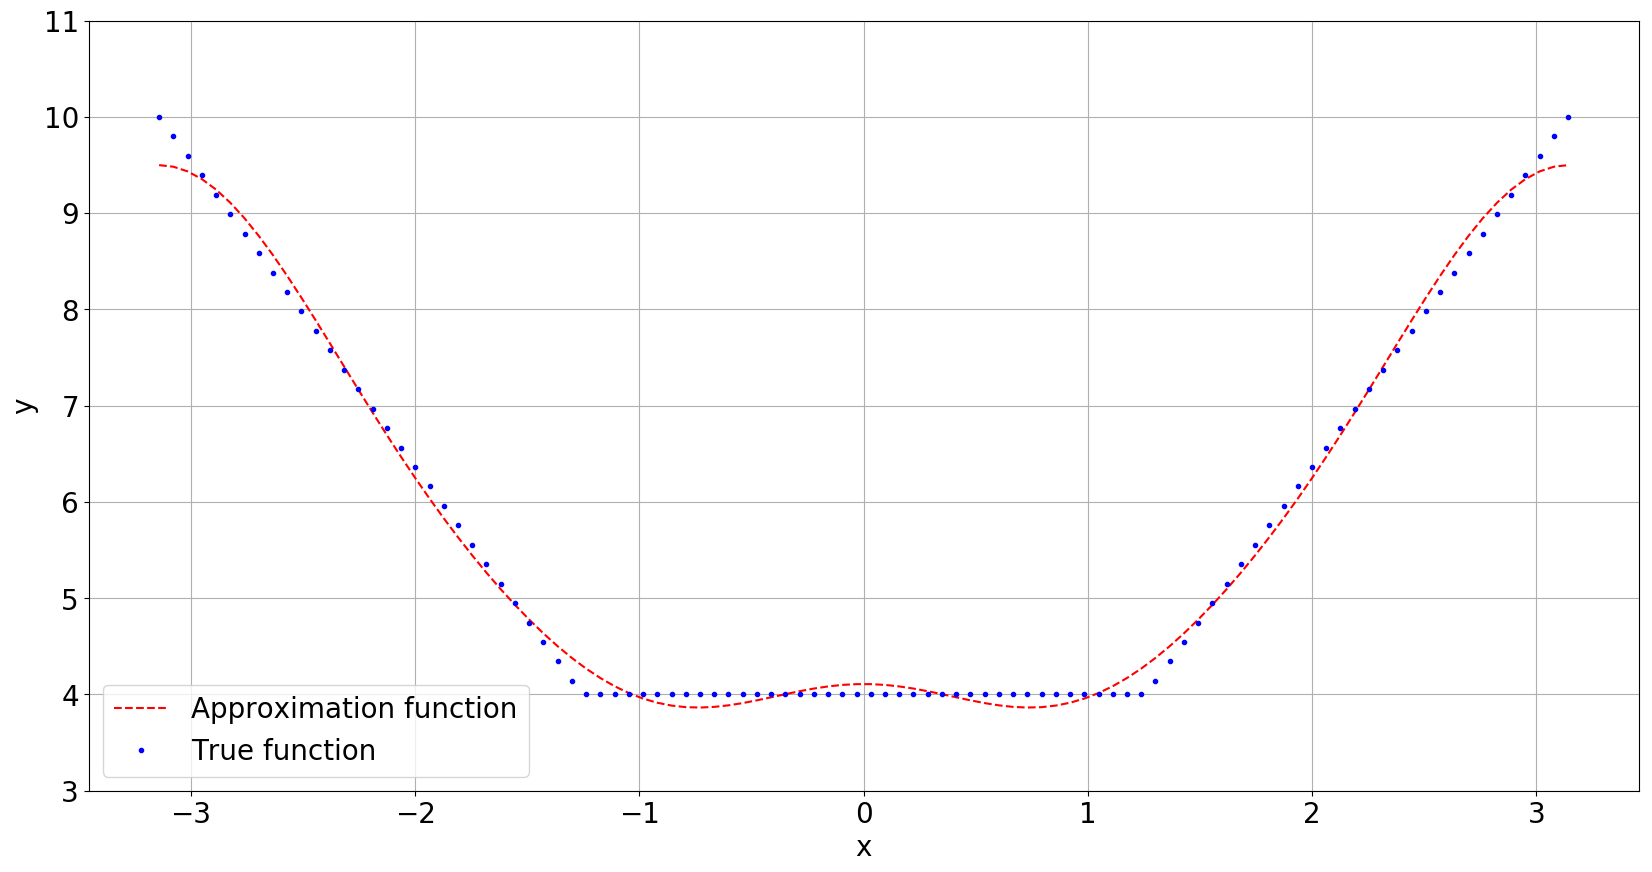
\includegraphics[width=\textwidth]{trigonometric.png}
\end{figure}
Порахуємо відхилення на $[-\pi, \pi]$ за формулою \eqref{delta} та отримуємо: \[ \Delta^2(f) = \texttt{0.10740063553045082}. \] Відхилення на $[-10, 10]$ дорівнює: \[ \Delta^2(f) = \texttt{0.341866841}. \]

\newpage

\subsubsection{Поліноми Чебишева}

Система функцій --- $\phi_n(x) = \cos (n \cdot \arccos(x))$, ортогональні з множником $\rho(x) = \dfrac{1}{\sqrt{1 - x^2}}$ на $[-1,1]$.

\begin{figure}[H]
    \centering
    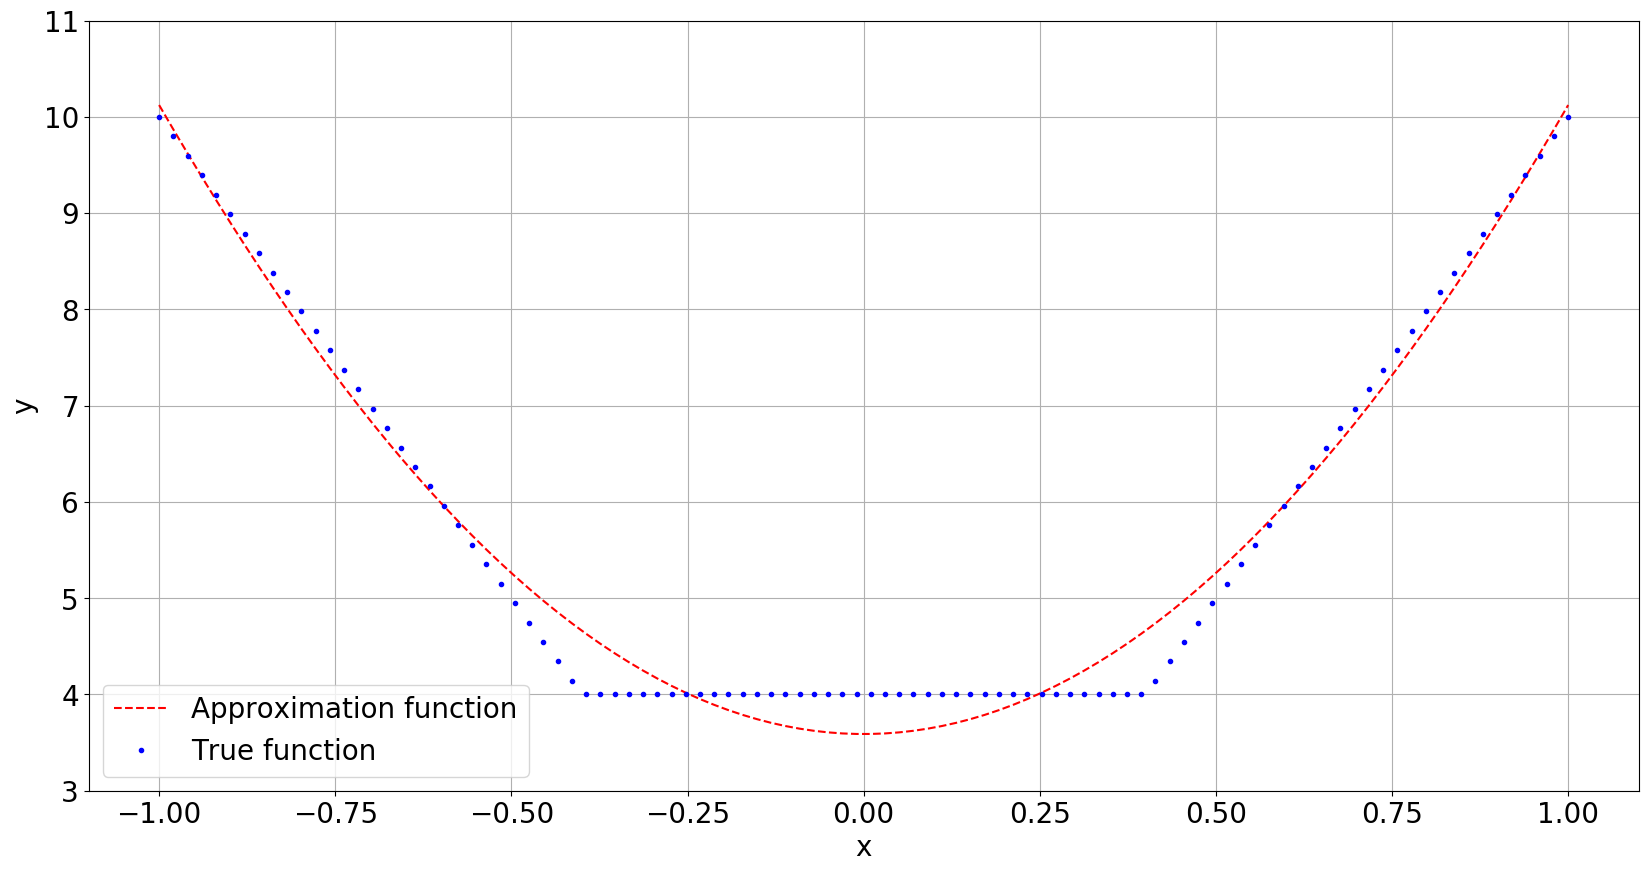
\includegraphics[width=\textwidth]{chebyshev.png}
\end{figure}
Порахуємо відхилення на $[-1, 1]$ за формулою \eqref{delta} та отримуємо: \[ \Delta^2(f) = \texttt{0.135158947199864}. \] Відхилення на $[-10, 10]$ дорівнює: \[ \Delta^2(f) = \texttt{1.35158947199864}. \]

\subsection{Метод найменших квадратів}

Нехай дано точки що ділить відрізок $[-10, 10]$ на 20 рівних частин та значення функції в них:

\begin{table}[H]
    \centering
    \begin{tabular}{|c|c|c|c|c|c|c|c|c|c|c|} \hline
        $i$ & 0 & 1 & 2 & 3 & 4 & 5 & 6 & 7 & 8 & 9 \\ \hline
        $x_i$ & $-10$ & $-9$ & $-8$ & $-7$ & $-6$ & $-5$ & $-4$ & $-3$ & $-2$ & $-1$ \\ \hline 
        $y_i$ & 10 & 9 & 8 & 7 & 6 & 5 & 4 & 4 & 4 & 4 \\ \hline
    \end{tabular}
    \break
    \hfill 
    \break
    \begin{tabular}{|c|c|c|c|c|c|c|c|c|c|c|c|} \hline
        $i$ & 10 & 11 & 12 & 13 & 14 & 15 & 16 & 17 & 18 & 19 & 20 \\ \hline
        $x_i$ & 0 & 1 & 2 & 3 & 4 & 5 & 6 & 7 & 8 & 9 & 10 \\ \hline
        $y_i$ & 4 & 4 & 4 & 4 & 4 & 5 & 6 & 7 & 8 & 9 & 10 \\ \hline
    \end{tabular}
\end{table}

Знайдемо значення похибки для різних $n$:

\begin{table}[H]
    \tt
    \centering
    \begin{tabular}{|c|c|} \hline
        $n$ & $\sigma_n$ \\ \hline
         1 & 0.2456140350877193000 \\ \hline 
         2 & 0.0044225627749655220 \\ \hline 
         3 & 0.0046827135264340820 \\ \hline 
         4 & 0.0049553959299550900 \\ \hline 
         5 & 0.0052857556586187624 \\ \hline 
         6 & 0.0024510823676256372 \\ \hline 
         7 & 0.0026396271651353016 \\ \hline 
         8 & 0.0008506324753000206 \\ \hline 
         9 & 0.0009279627003272911 \\ \hline 
        10 & 0.0007896501165176935 \\ \hline 
        11 & 0.0008773890183529924 \\ \hline 
        12 & 0.0008200149552223944 \\ \hline 
        13 & 0.0009371599488255855 \\ \hline 
        14 & 0.0004570848289908443 \\ \hline 
    \end{tabular}
\end{table}

Поліном найкращого середньоквадратичного наближення оптимального степеня та отримуємо, що $m = m^\star = 8$, тобто з моменту коли наступна величина стабілізується або почне зростати: \[\sigma^2 = \sqrt{\frac{1}{n - m} \sum_{k = 0}^n (P_m(x_k) - y_k)^2}.\] 

\begin{figure}[H]
    \centering
    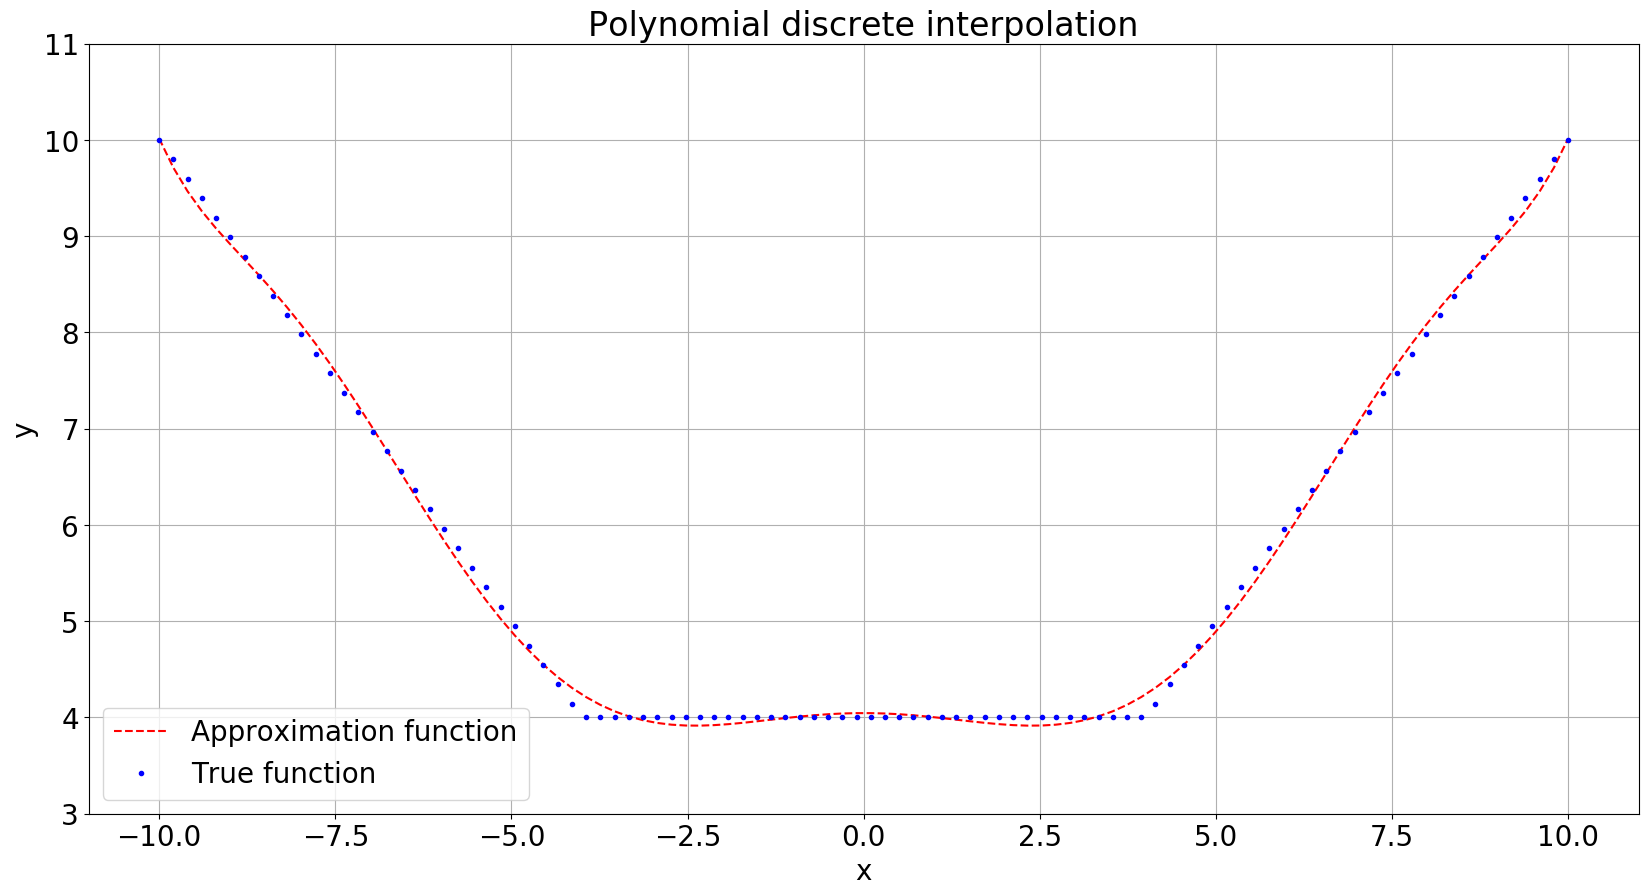
\includegraphics[width=\textwidth]{discrete.png}
\end{figure}

Відповідна ``похибка'' (у лапках бо взята із ваговим коефіцієнтом): \[ \sigma_2 = \texttt{0.0008506324753000206}. \]


\subsection{Кубічні згладжувальні сплайни}

Будуємо кубічний сплайн для $n = 15$ та різних $\rho$.

\begin{figure}[H]
    \centering
    \includegraphics[width=\textwidth]{{spline_1}.png}
\end{figure}

Відхилення на $[-10, 10]$ дорівнює: \[ \Delta^2(f) = \texttt{0.15336142100936748}. \]

\begin{figure}[H]
    \centering
    \includegraphics[width=\textwidth]{{spline_0.003}.png}
\end{figure}

Відхилення на $[-10, 10]$ дорівнює: \[ \Delta^2(f) = \texttt{18.429578862891297}. \]

\begin{figure}[H]
    \centering
    \includegraphics[width=\textwidth]{{spline_300.0}.png}
\end{figure}

Відхилення на $[-10, 10]$ дорівнює: \[ \Delta^2(f) = \texttt{0.012596258104766956}. \]

\end{document}
